\begin{figure}[h]
    \centering
    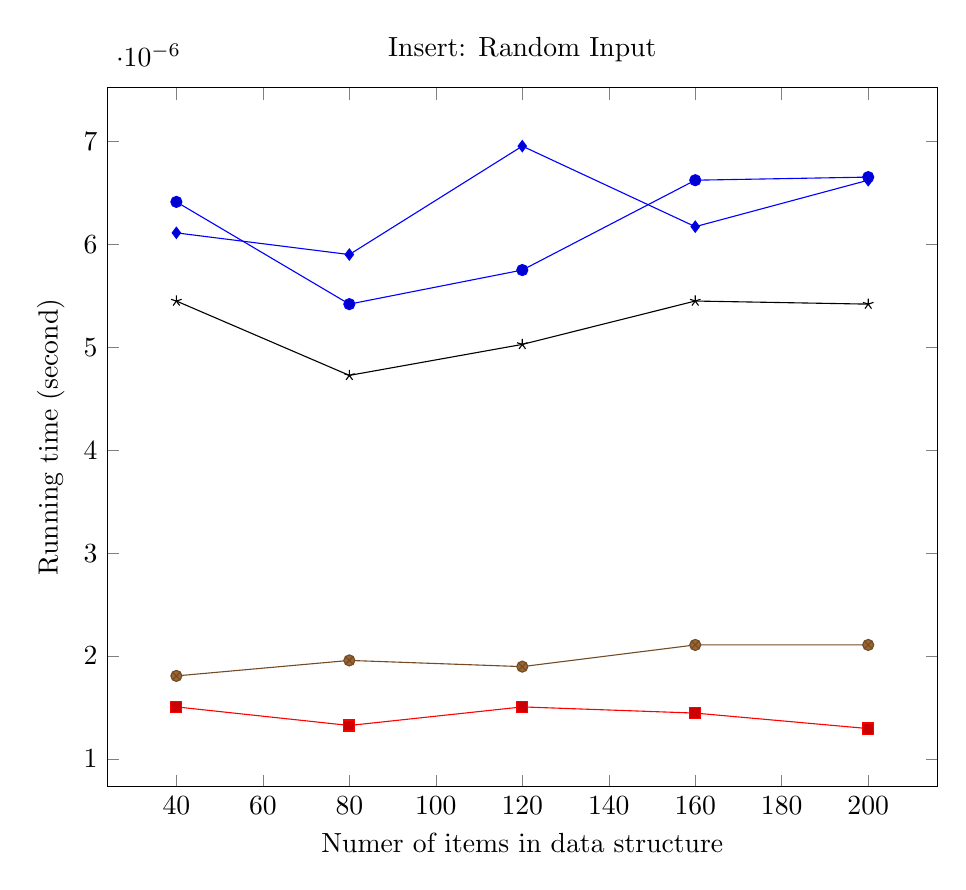
\begin{tikzpicture}
        \begin{axis}[
            xlabel={Numer of items in data structure},
            ylabel={Running time (second)},
            title={Insert: Random Input},
            width=\textwidth
        ]
		\addplot coordinates {
			(40, 6.415034672713204e-06)
			(80, 5.421156061657939e-06)
			(120, 5.752448931772846e-06)
			(160, 6.6258574086930365e-06)
			(200, 6.65597494204917e-06)
		};
		\addplot coordinates {
			(40, 1.505876683793872e-06)
			(80, 1.3251714818807159e-06)
			(120, 1.5058766834386005e-06)
			(160, 1.445641616726334e-06)
			(200, 1.29505394781404e-06)
		};
		\addplot coordinates {
			(40, 1.8070520205526463e-06)
			(80, 1.957639689109669e-06)
			(120, 1.8974046213315888e-06)
			(160, 2.1082273573114206e-06)
			(200, 2.1082273573114206e-06)
		};
		\addplot coordinates {
			(40, 5.4512735953693435e-06)
			(80, 4.728452787006176e-06)
			(120, 5.029628123764951e-06)
			(160, 5.4512735950140724e-06)
			(200, 5.421156061657939e-06)
		};
		\addplot coordinates {
			(40, 6.11385933595443e-06)
			(80, 5.903036600329869e-06)
			(120, 6.957150278807944e-06)
			(160, 6.17409440337724e-06)
			(200, 6.6258574083377654e-06)
		};
        \legend{}
        \end{axis}
    \end{tikzpicture}
    \caption{Average of 0 operations, benchmarked every 0, starting at 0.}
\end{figure}